
%%% Local Variables:
%%% mode: latex
%%% TeX-master: t
%%% End:

% !Mode:: "TeX:UTF-8"

\chapter{动态温度与功耗管理系统的模拟验证}
\label{cha:DPTMexperiments}

\section{模拟实验环境}
为了验证本文所提出的预测任务负载模型、VP-TALk调度算法以及DPTM原型系统,我们进行了三组模拟实验。实验运行平台为配有Intel Core 2 Q9550 CPU、4GB RAM的Windows7 64位操作系统,预测模型以及各DPTM算法在MATLAB\onlinecite{MATLAB}软件中进行仿真模拟。

\section{VP-TALk算法的动态温度与功耗管理效果验证}
本文通过与现有的TALk、PB、MO算法进行对比,来验证本文提出的VP-TALk算法的优越性。 实验中选取$p_r$、$c_r$取值分别为0.001$s$/$V$和0.01$J$/$V^2$,温度最高上限设为390K,任务周期固定为10$s$。 支持DVFS芯片的电压值从0.6$V$到1.4$V$可调,步长0.1$V$。根据电压可以得到归一化的速度序列为{0.574, 0.6611, 0.7324, 0.7926, 0.8446, 0.8901, 0.930, 0.9670, 1}。 任务负载率为5\%至95\%,变化步长为5\%。 对于4种对比算法,我们分别将能耗情况(单位为焦耳$J$)和峰值温度情况(单位为绝对温度$K$)绘制于 图\ref{fig:vp-talk-power-cmp}和图\ref{fig:vp-talk-temp-cmp}。
\begin{figure}[H]
  \centering
  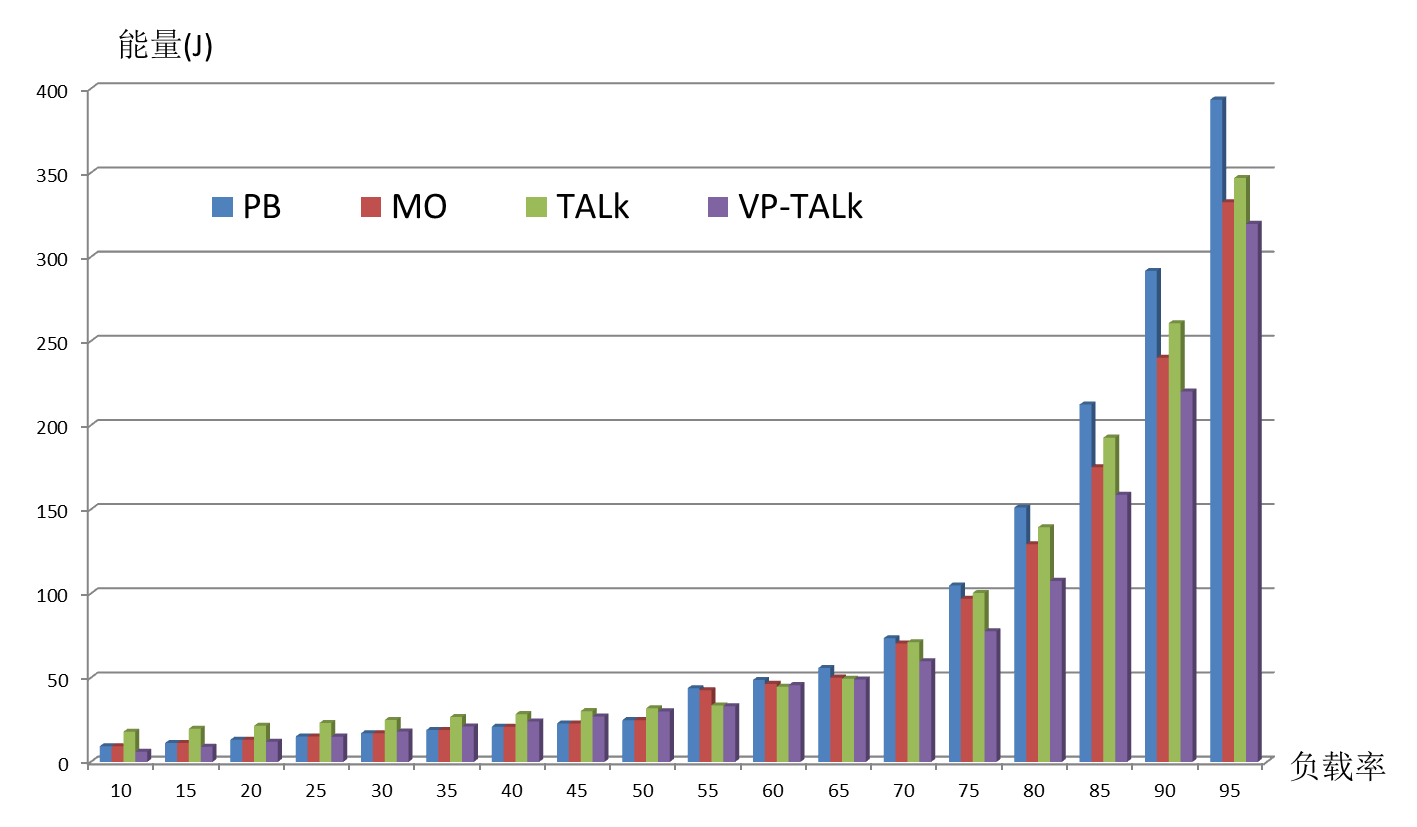
\includegraphics[width=0.8\textwidth,height=0.4\textheight]{VP-TALK-POWER-CMP}
  \caption{各种算法的能耗调度效果比较}
  \label{fig:vp-talk-power-cmp}
\end{figure}
\begin{figure}[H]
  \centering
  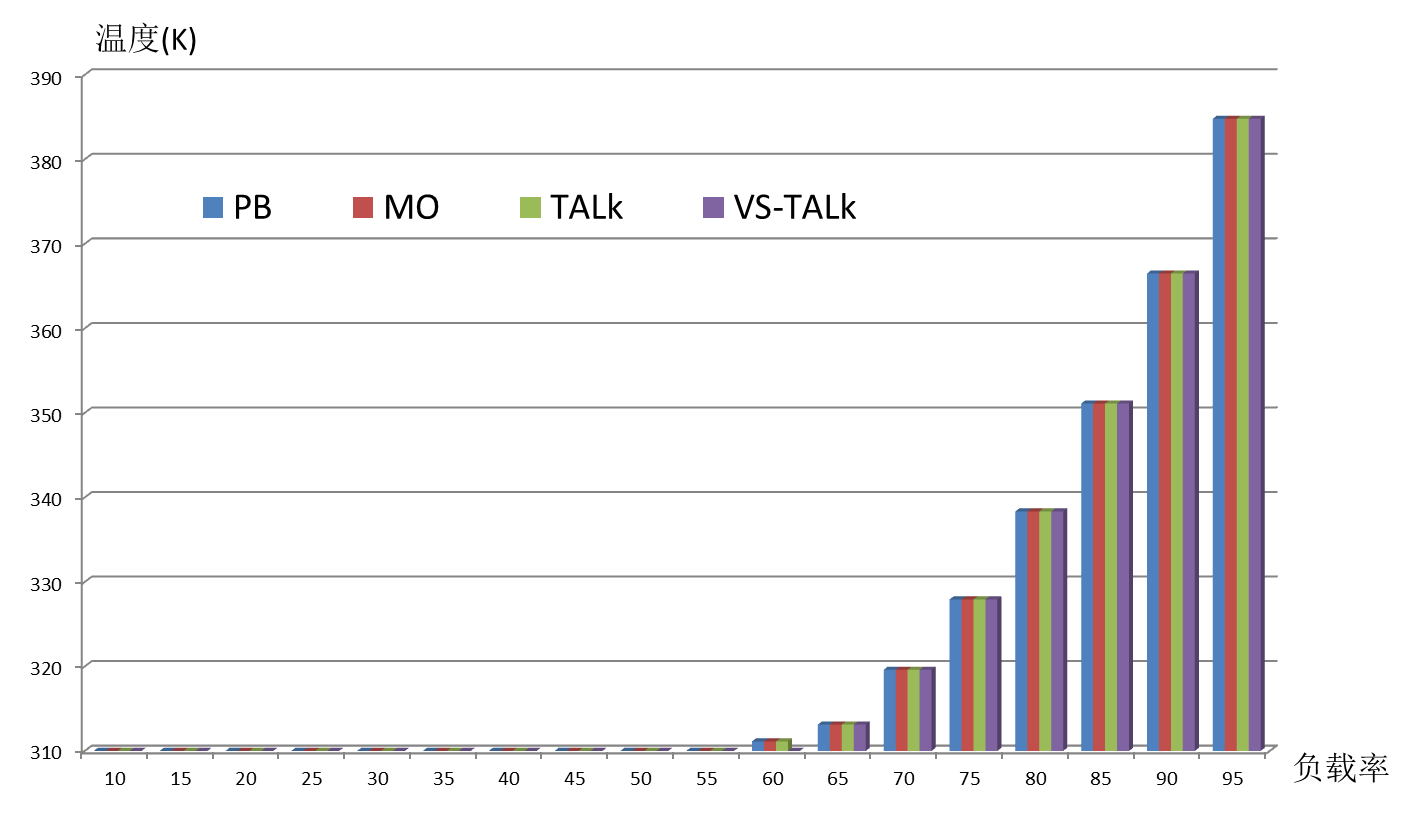
\includegraphics[width=0.8\textwidth,height=0.4\textheight]{VP-TALK-TEMP-CMP}
  \caption{各种算法的峰值温度调度效果比较}
  \label{fig:vp-talk-temp-cmp}
\end{figure}
从图\ref{fig:vp-talk-power-cmp}可以看出,对于能耗:当负载率小于55\%时,VP-TALk优于TALk、PB与MO等价。 这是因为,在负载率不高于芯片最低运行速度(0.574)时,VP-TALK相当于使用DVS技术的TALk,PB相当于使用单一速度的MO。 此时,TALk与PB的调度效果相差无几。在负载率为25\%到50\%时,PB略优于VP-TALk算法。 原因是VP-TALk在电压和时间切换上付出了更大的代价。 然而,随着负载率的增加,当负载率大于55\%时,VP-TALk的调度效果全面优于其他三种算法, 比PB、MO以及TALk的平均能耗分别节省大约20.54\%、11.04\%、11.42\%。表\ref{tab:chap3:vp-talk-cmp}列出了当负载率大于55\%时,能耗节省数据的统计信息, 具体说明了VP-TALk的在能耗节约方面的优势。
从图\ref{fig:vp-talk-temp-cmp}中可以看出,当工作负载率小于50\%时,各种算法所达到的峰值温度都不超过310$K$, 四种调度算法在峰值温度方面的差距基本小于1$K$,并在最大负载率时近似共同终结于384$K$。

\begin{table}
\centering
\caption{VP-TALk算法调度效果与已有算法的比较}
\begin{tabular}{c c c c c}
\hline\hline
算法 & PB & MO & TALk & Avg \\ [0.5ex]
\hline
平均(\%) & 20.54 & 11.04 & 11.42 & 14.33 \\
最大(\%) & 28.83 & 22.34 & 21.27 & 24.68 \\
\hline
\end{tabular}
\label{tab:chap3:vp-talk-cmp}
\end{table}

\section{基于在线评价的动态温度与功耗管理系统的效果评测}
为了评价本文基于机器学习的实时功耗温度管理原型系统功耗与温度的调度效果,我们做了两组实验。
首先,基于\onlinecite{DPTMbyYJQ}中所得到的每个时刻工作负载预测值,我们分别采用四种对比源算法, 即TALk\onlinecite{TemLkMinTechRTSys}、PB\onlinecite{EngRTTskSchTemDepLk}、 MO\onlinecite{LkEngMinRTSysMaxTemConst},VP-TALk, 算出每个时刻每种算法的能耗值与峰值温度; 然后将四种对比源算法每个时刻的能耗值与峰值温度进行平均,得到四种对比源算法每个时刻的平均调度效果; 最后使用图\ref{fig:dptm-source-alg-power-cmp}与图\ref{fig:dptm-source-alg-temp-cmp}分别 比较了本文原型系统与四种对比源算法平均调度效果的能耗(单位$J$)和峰值温度(单位$\celsius$)。
\begin{figure}[H]
  \centering
  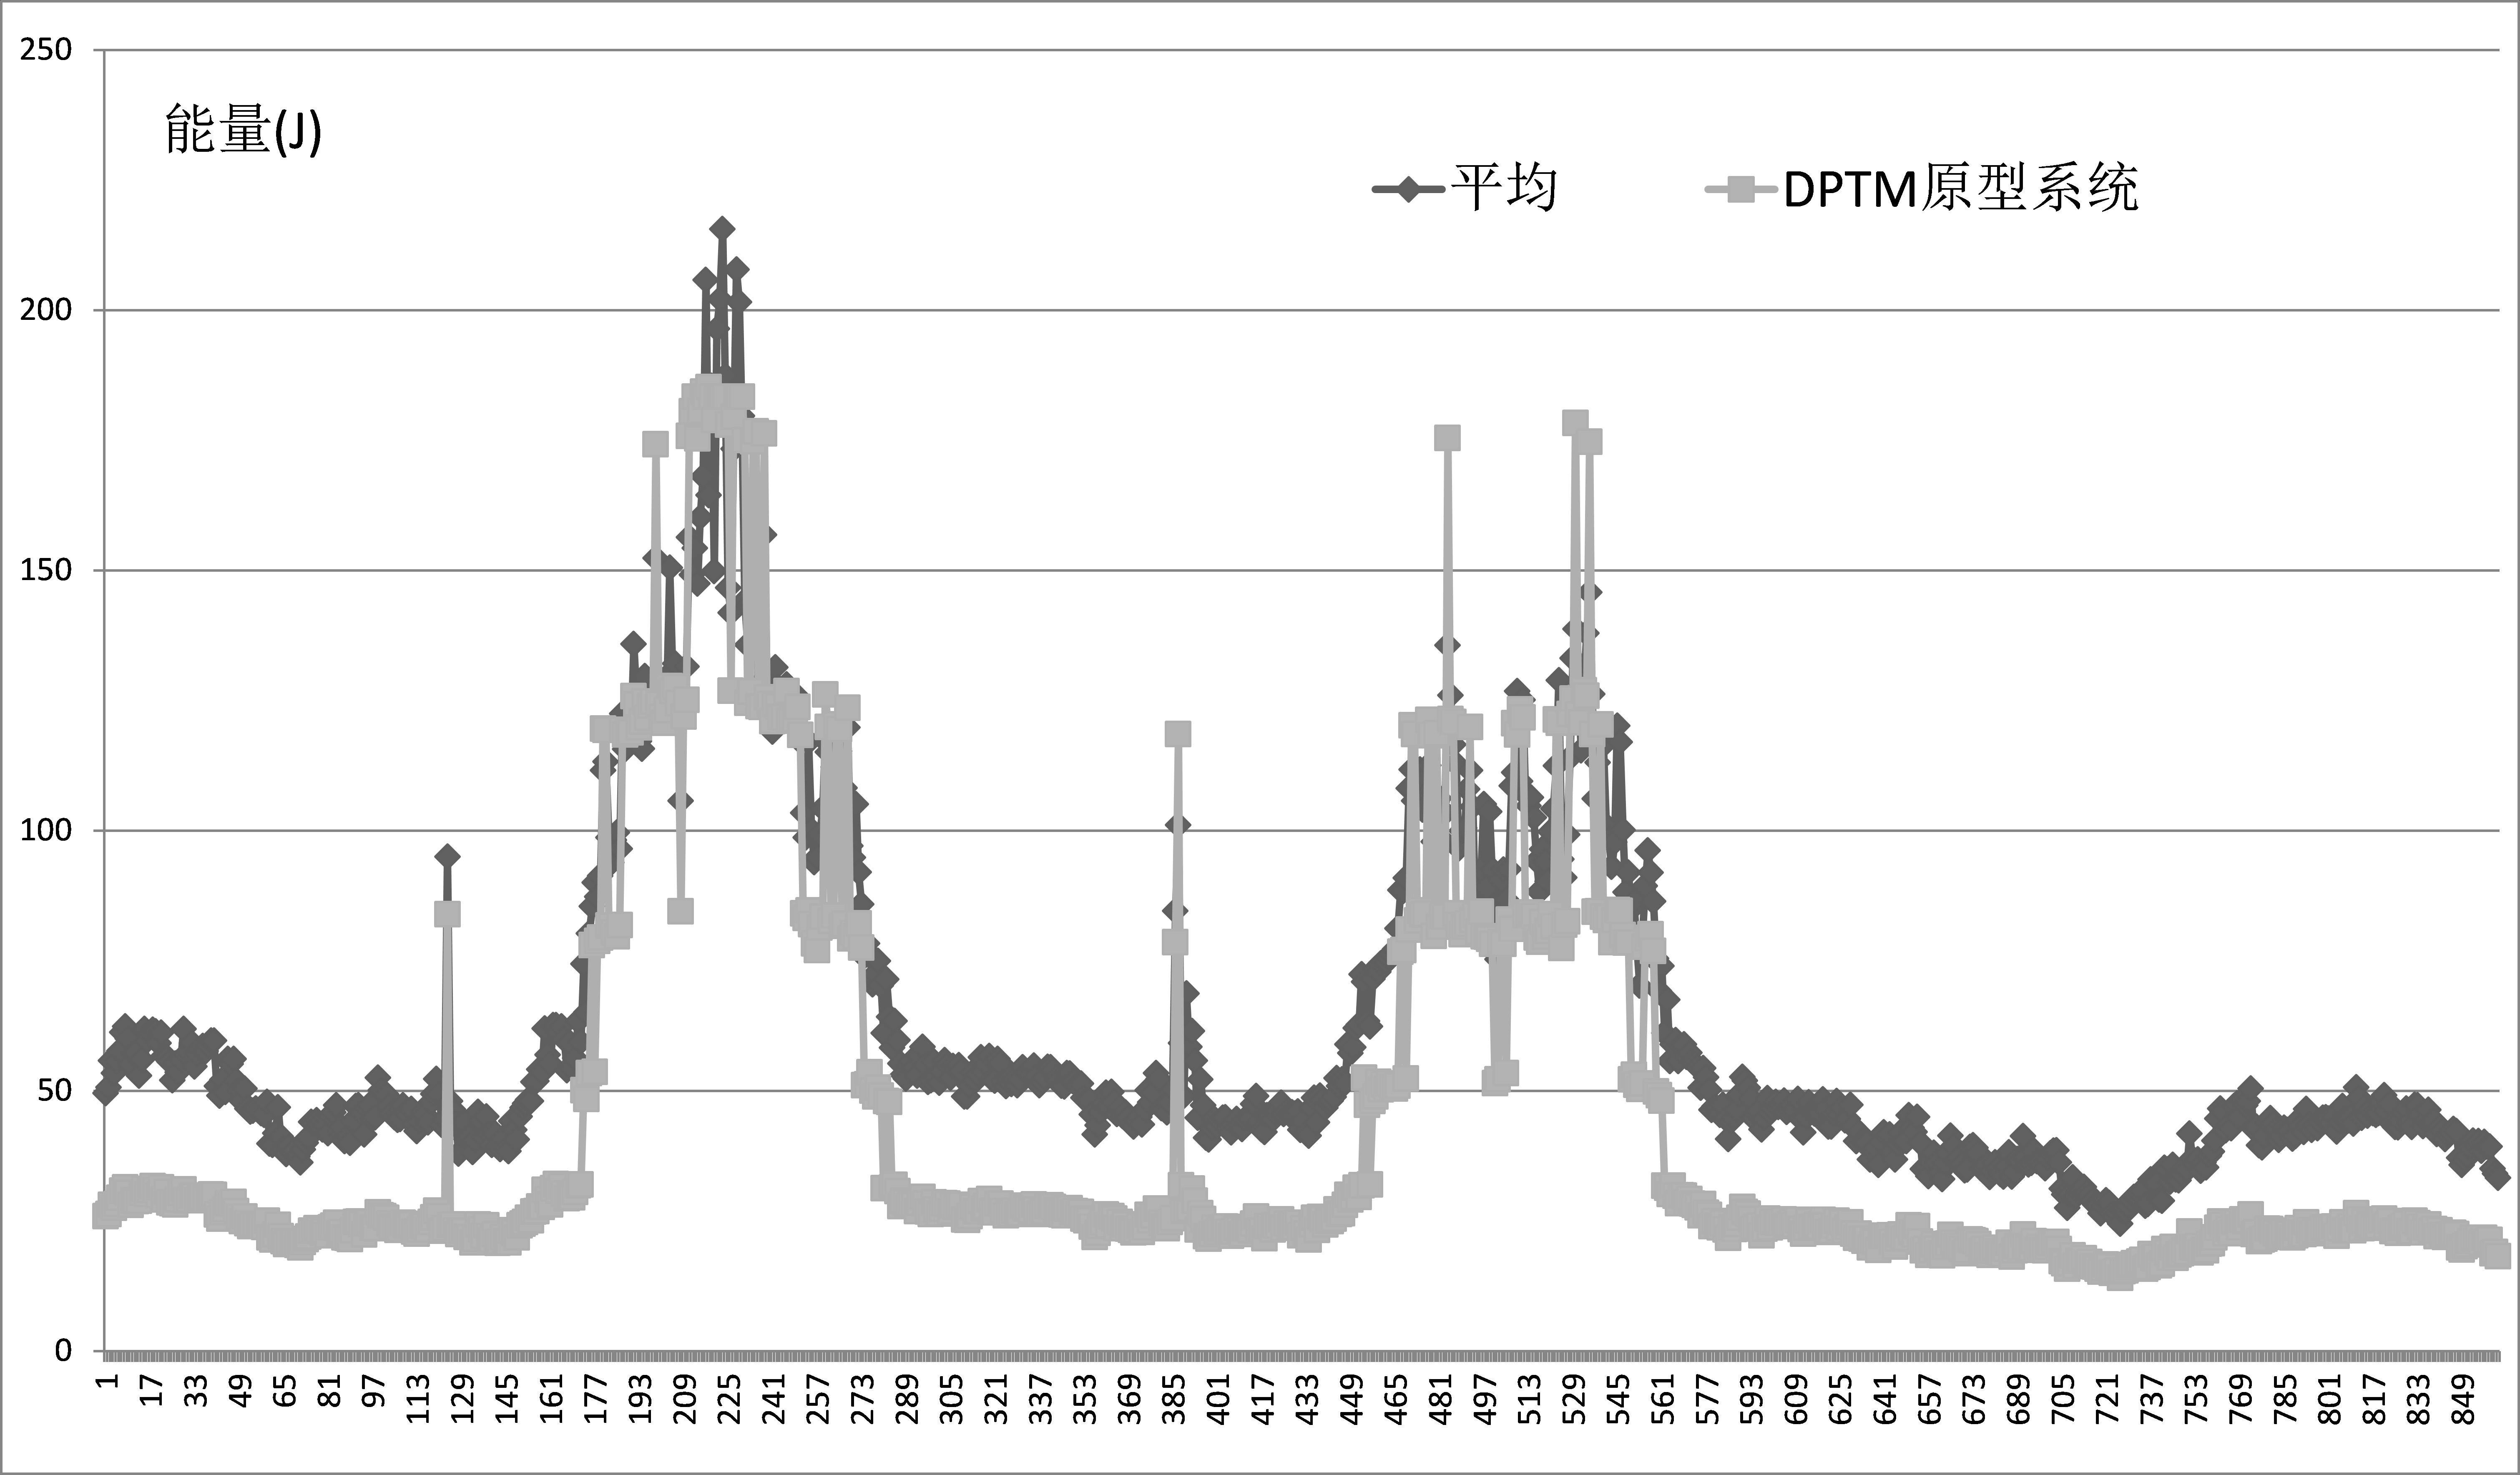
\includegraphics[width=1.0\textwidth,height=0.4\textheight]{DPTM-SOURCE-ALG-POWER-CMP}
  \caption{基于在线评价的动态温度与功耗管理系统VS各种源算法均值(能耗调度效果)}
  \label{fig:dptm-source-alg-power-cmp}
\end{figure}
\begin{figure}[H]
  \centering
  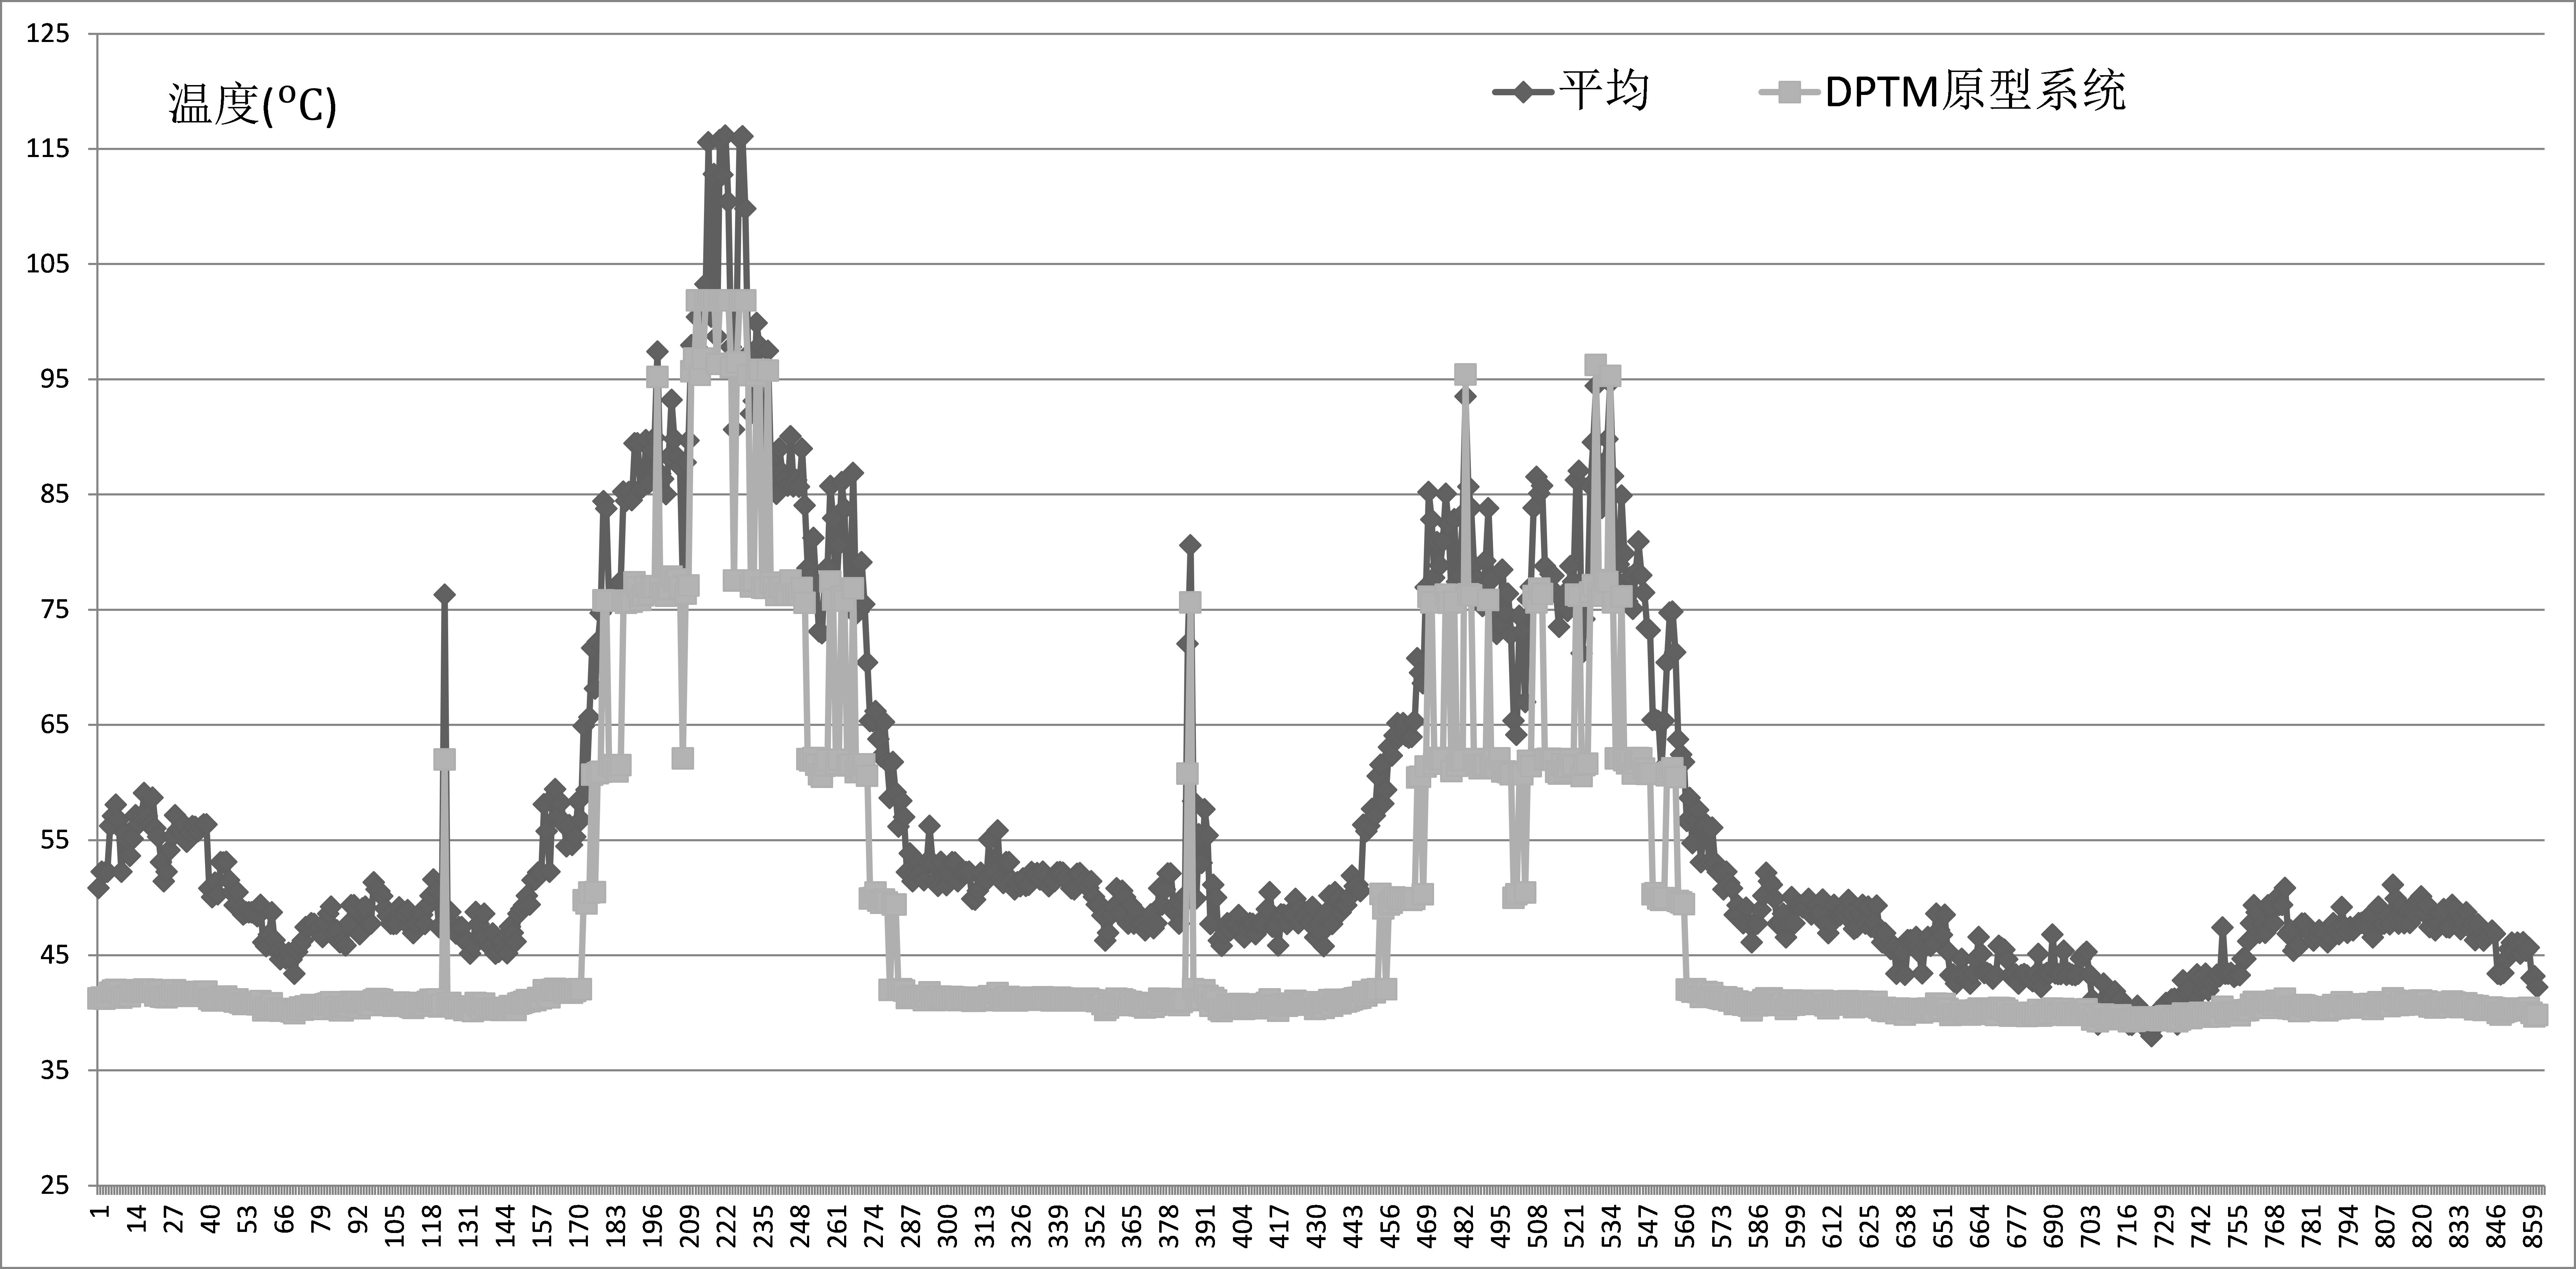
\includegraphics[width=1.0\textwidth,height=0.4\textheight]{DPTM-SOURCE-ALG-TEMP-CMP}
  \caption{基于在线评价的动态温度与功耗管理系统VS源算法均值(峰值温度调度效果)}
  \label{fig:dptm-source-alg-temp-cmp}
\end{figure}
\begin{figure}[H]
  \centering
  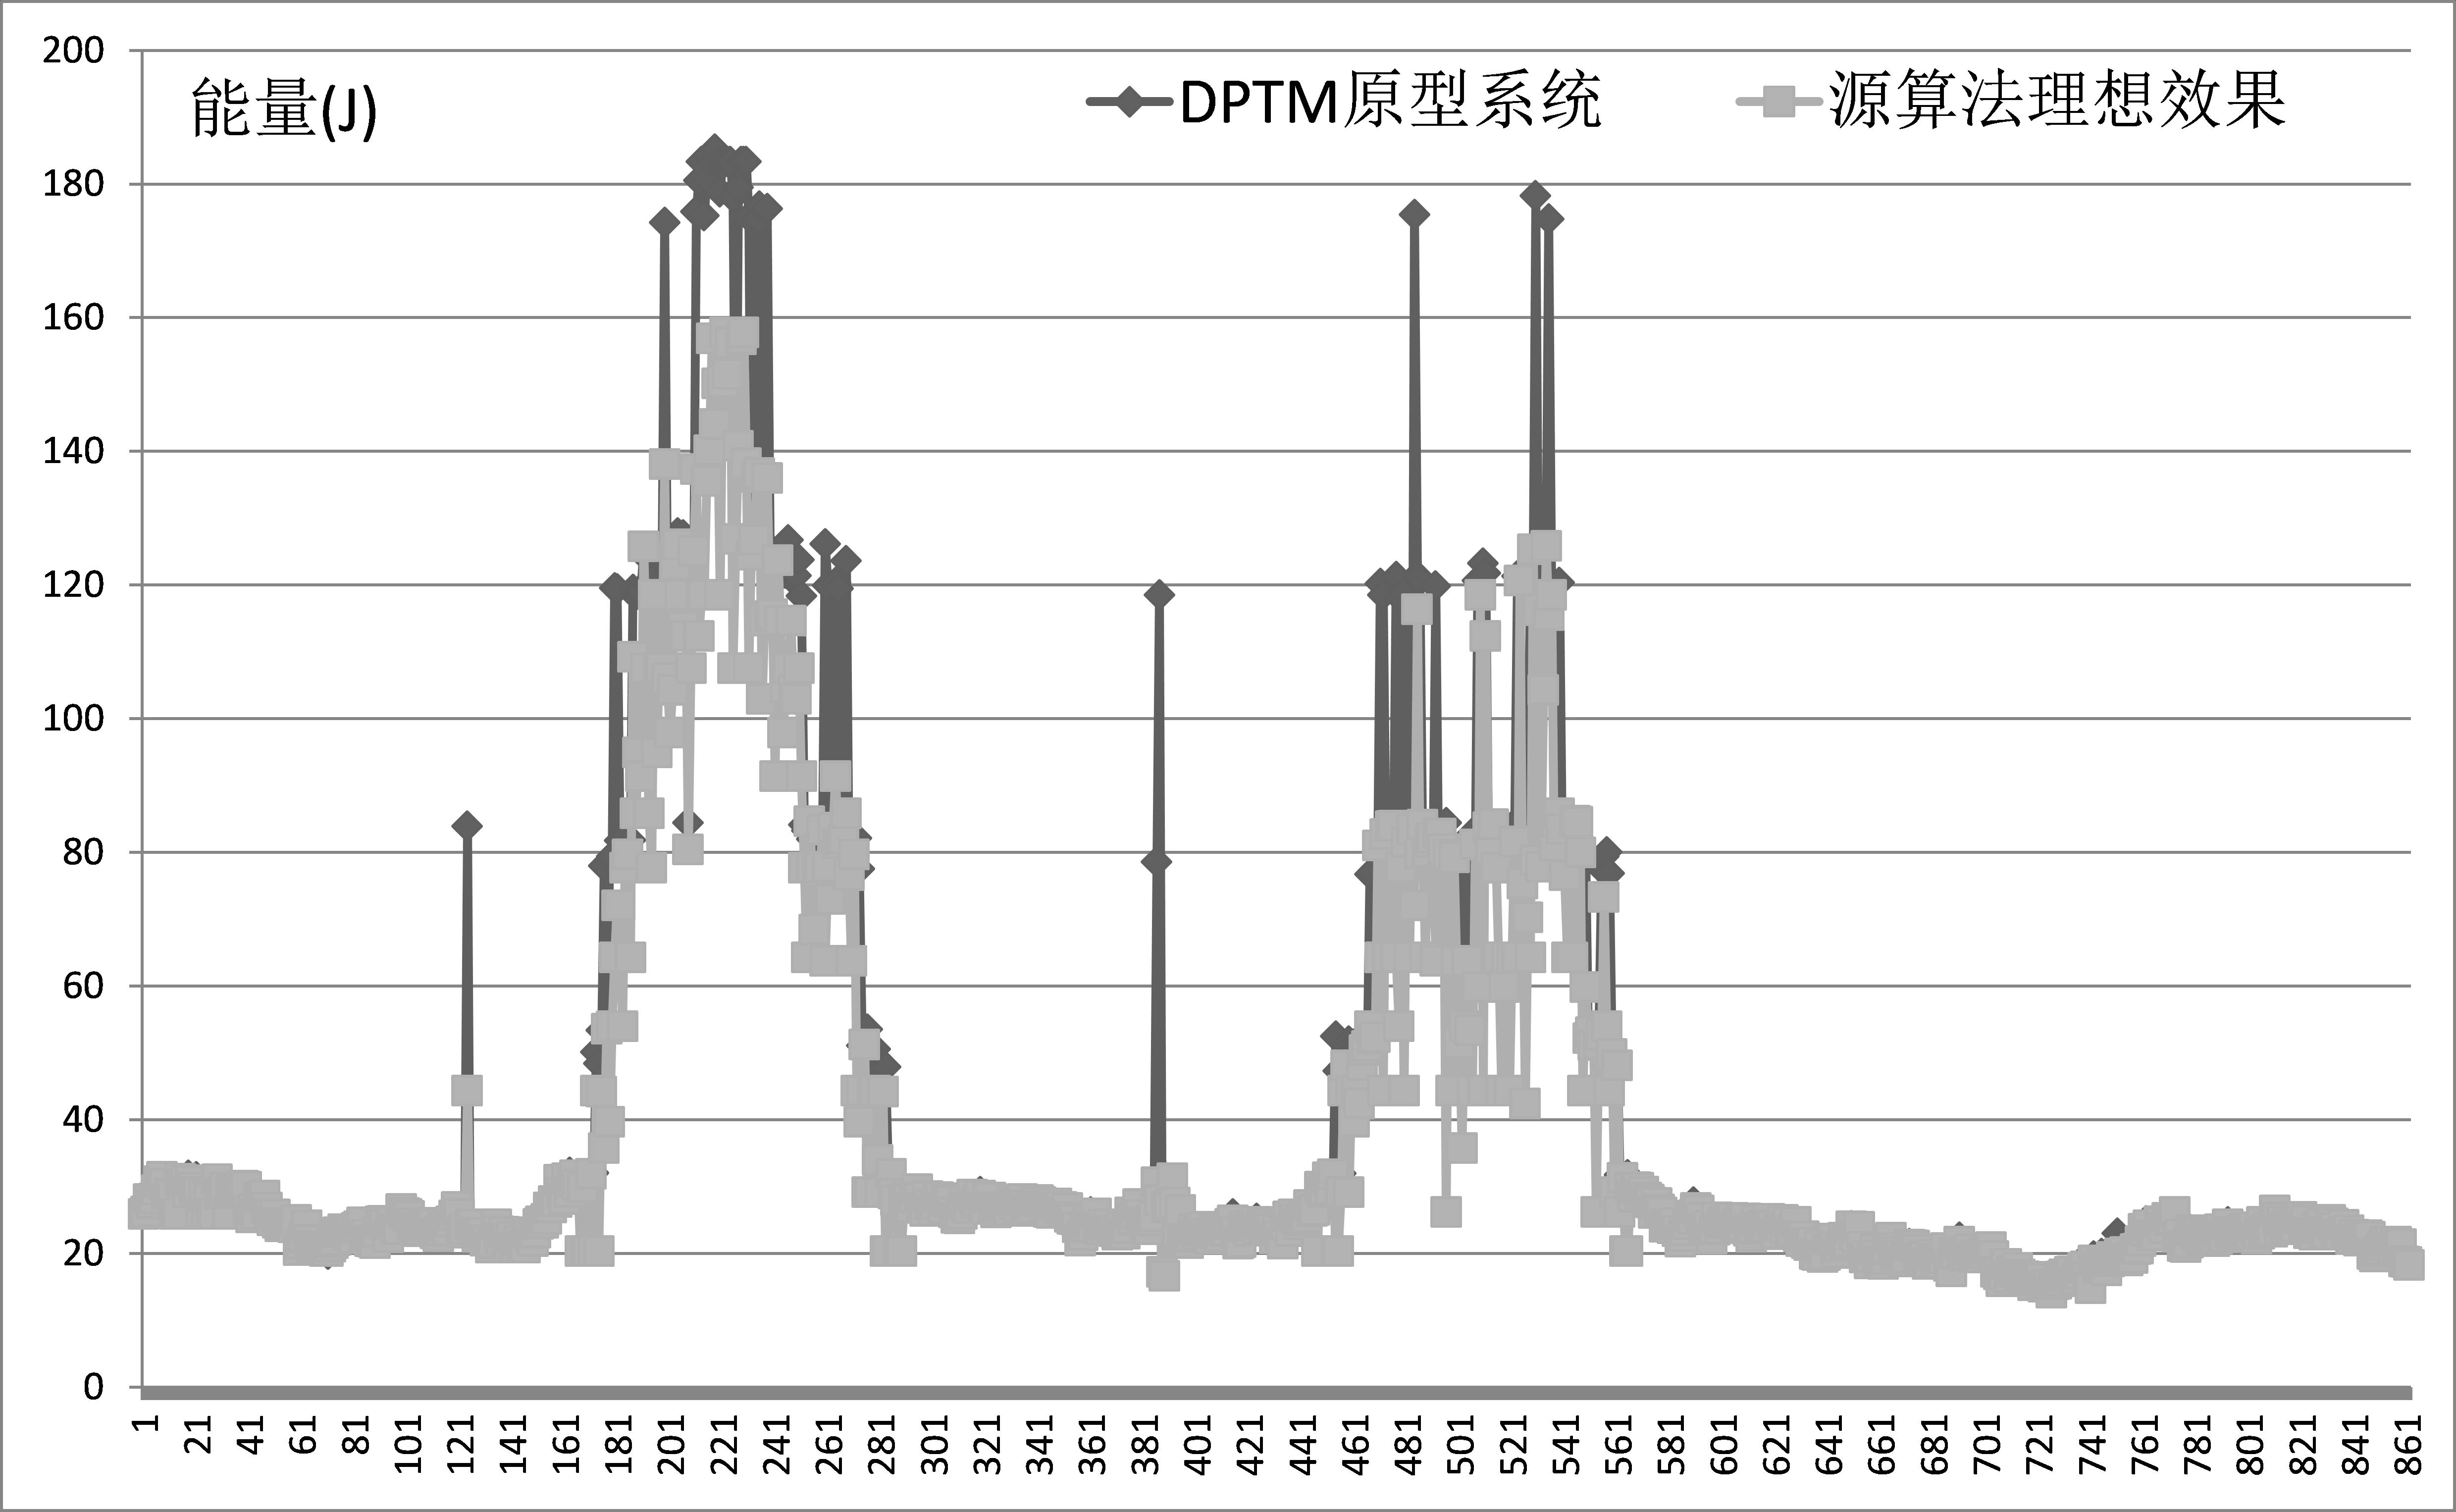
\includegraphics[width=1.0\textwidth,height=0.4\textheight]{DPTM-IDEAL-POWER-CMP}
  \caption{基于在线评价的动态温度与功耗管理系统VS理想调度效果(能耗调度效果)}
  \label{fig:dptm-ideal-power-cmp}
\end{figure}
\begin{figure}[H]
  \centering
  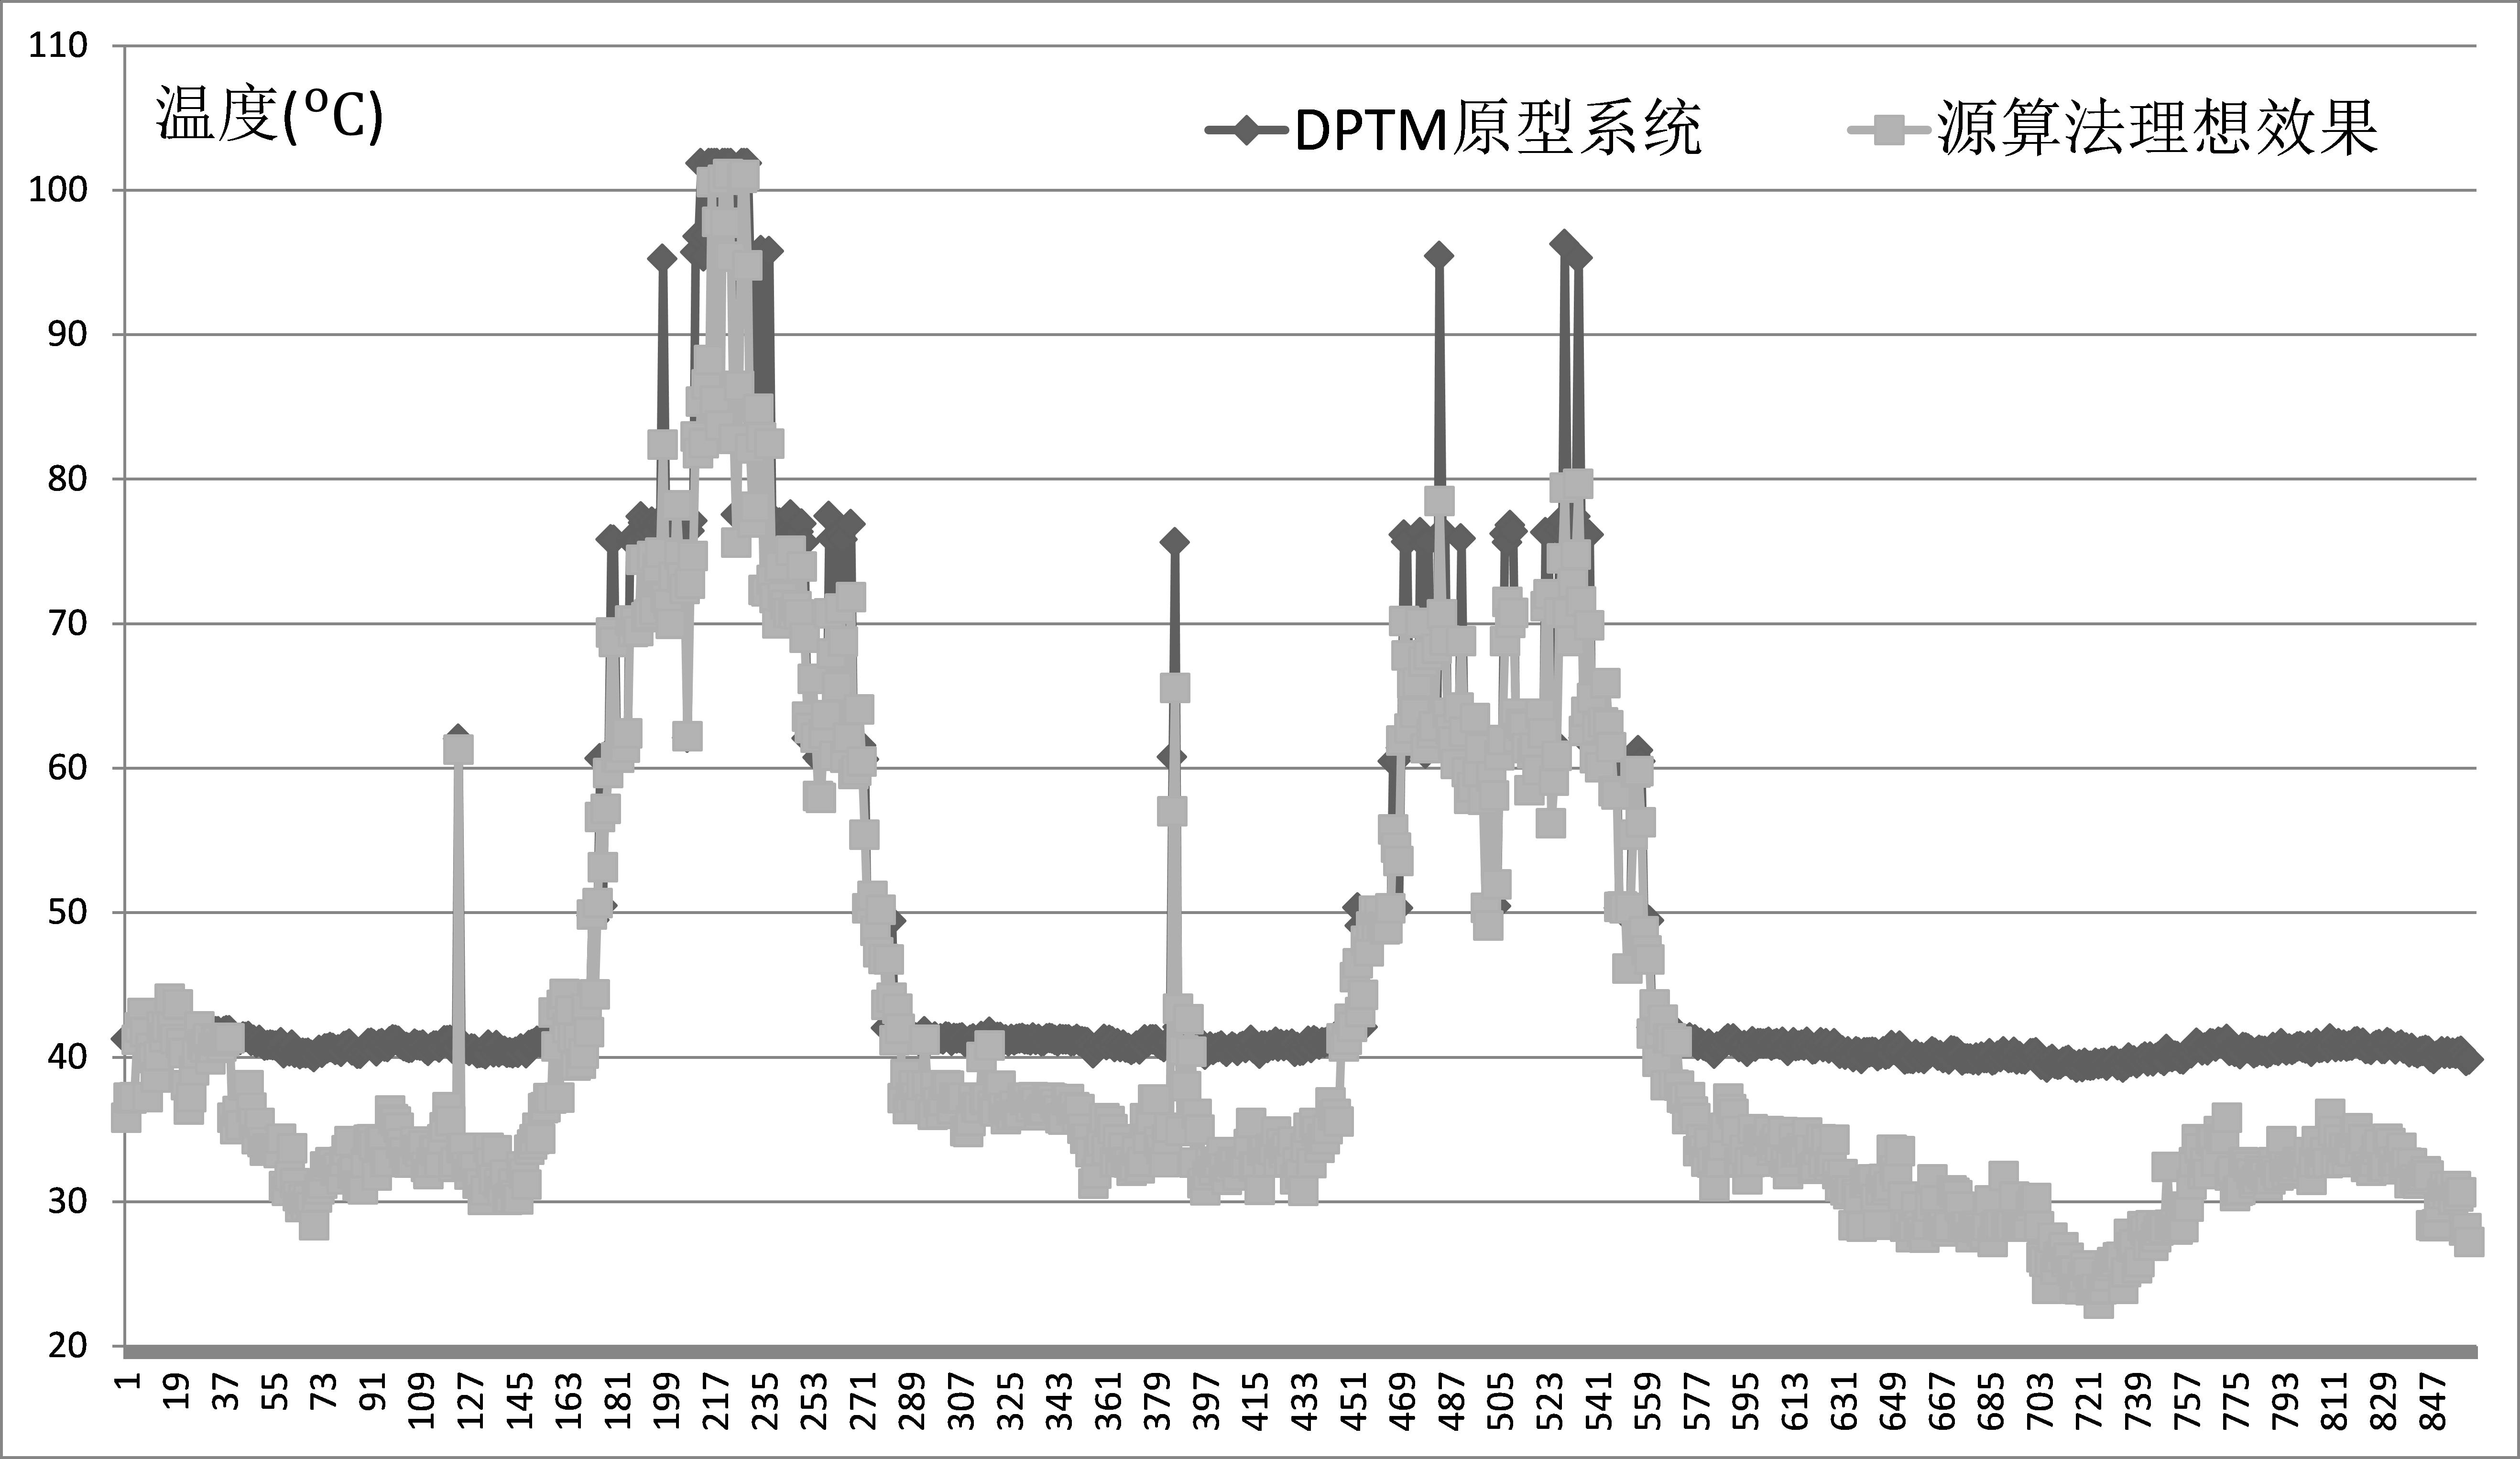
\includegraphics[width=1.0\textwidth,height=0.4\textheight]{DPTM-IDEAL-TEMP-CMP}
  \caption{基于在线评价的动态温度与功耗管理系统VS理想调度效果(峰值温度调度效果)}
  \label{fig:dptm-ideal-temp-cmp}
\end{figure}

其次,同样基于\onlinecite{DPTMbyYJQ}中所得到的每个时刻工作负载真实值,采用四种源算法,分别算出每个时刻的能耗值与峰值温度, 取其中的最优值作为实时功耗温度管理调度的理想值; 然后使用这批理想值来客观评价集成了TALk、PB、MO以及VP-TALk算法的实时功耗温度管理原型系统的调度效果; 最后使用图\ref{fig:dptm-ideal-power-cmp}与图\ref{fig:dptm-ideal-temp-cmp}分别 比较了本文原型系统与四种对比源算法理论最优调度效果的能耗(单位$J$)和峰值温度(单位$\celsius$)。
从图\ref{fig:dptm-source-alg-power-cmp}与图\ref{fig:dptm-source-alg-temp-cmp}可以直观地看出: 与四种源算法平均调度效果相比, 本文原型系统择优式的组合DPTM算法可以明显拉低实时系统的运行能耗曲线和峰值温度曲线, 这表明对比于四种DPTM源算法,本文基于机器学习的实时功耗温度管理原型系统获得了"取其长、去其短"的优化效果。 同时从表3的比较数据可以得出"本文原型系统可以获得近似最优的调度效果"的结论,其实验依据如下:
\begin{enumerate}[1)]
\item 与四种DPTM源算法的平均效果相比(图\ref{fig:dptm-source-alg-power-cmp}), 本文原型系统采用的择优式组合DPTM算法可获得更优的能耗优化效果, 所有时间采样点能耗的累加值$E_{TOTAL}$(总能耗)可获得18.39\%的改进, 所有时间采样点中的最大值$E_{MAX}$(最大能耗)可获得18.77\%的改进。整体改进效果非常明显。
\item 与四种DPTM源算法相比(图\ref{fig:dptm-source-alg-temp-cmp}),本文原型系统可以获得更优的峰值温度优化效果, 所有时间采样点中的最大峰值温度$T_{PMAX}$是最优, 所有时间采样点峰值温度的平均值$T_{PAVG}$是比算法均值稍弱。与四种DPTM源算法调度效果平均值相比, 本文原型系统可以获得$T_{PMAX}$1.81$\celsius$的改进,但$T_{PAVG}$ 有-1.31$\celsius$的退化。从拉低最大峰值温度的角度来讲,改进效果较为明显。
\item 通过图\ref{fig:dptm-ideal-power-cmp}与图\ref{fig:dptm-ideal-temp-cmp} 对本文原型系统的调度效果与理想值进行的直观比较, 看出本文原型系统可以获得比四种源算法均值更接近于理想值的优化效果。 与表3中理想值的$E_{TOTAL}/E_{MAX}/T_{PAVG}/T_{PMAX}$参数相比, 四种DPTM源算法调度效果平均值会产生28.64\%/30.09\%/7.71$\celsius$/9.73$\celsius$的差距, 而本文原型系统只产生了12.55\%/13.93\%/9.02$\celsius$/7.91$\celsius$差距。
\end{enumerate}

\section{本章总结}
第\ref{cha:DPTM}章深入分析与评估了已有的主流调度算法,提出了一系列调度准则和经验。 基于这些对芯片工作休眠状态调度的经验准则,我们提出一种在能耗节省方面更具优势的DPTM调度算法VP-TALk, 以此算法为基础,综合本文所提出的预测任务负载模型,构建了一个基于负载预测的实时功耗温度管理系统。本章中的仿真实验表明,
\begin{enumerate}[1)]
\item 本文的组合模型在负载预测方面胜过众多的相关模型及算法,平均误差仅为2.89\%;
\item 本文所提出的VP-TALk算法在较高的工作负载率和共同的峰值温度约束下, 分别比Pattern-Based、M-Oscillating、TALk分别节能20.54\%、11.04\%、11.42\%;
\item 本文所提出的综合四种源算法、基于机器学习的实时功耗温度管理原型系统较为接近理想值, 与其$E_{TOTAL}/E_{MAX}/T_{PAVG}/T_{PMAX}$参数相比, 只产生了12.55\%/13.93\%/9.02$\celsius$/7.91$\celsius$差距。
\end{enumerate}
